\chapter{Metodología y Desarrollo}
\label{cap:descripcionTrabajo}


\section{Descripción del conjunto de datos (\textit{Dataset})}
 El conjunto de datos empleado está compuesto por imágenes de resonancia magnética nuclear (IRM) preclínicas de cerebros de ratón, obtenidas en el contexto de colaboración con el centro \textit{ICTS BioImagen Complutense}. Estas imágenes constituyen la base para el entrenamiento y evaluación de los modelos de segmentación automática de la estructura cerebral y las lesiones asociadas, en este caso, la lesión por isquemia cerebral.

 Tal y como se establece en los objetivos del proyecto, el dataset ha sido diseñado para permitir tanto la delimitación anatómica del cerebro como la identificación de regiones patológicas, lo que implica la coexistencia de dos tipos de anotaciones: segmentación de órgano sano y segmentación de lesión.
  
\subsection{Estructura del dataset}
El dataset presenta una estructura jerárquica, en la que cada caso de estudio se presenta en una carpeta individual con la denominación "\textit{CASE n}". 
Para cada caso, se dispone de los siguientes elementos:

\subsubsection{Volúmenes en formato NIfTI (\texttt{.nii})}
El formato \textbf{NIfTI} \textit{(Neuroimaging Informatics Technology Initiative)} es el estándar en neuroimagen por su capacidad de almacenar datos volumétricos junto a metadatos asociados, como se describe en la documentación oficial estándar \citep{nifti} .

Además, se ha decidido usar NIfTI frente a otros formatos debido a que es uno de los estándares más utilizados en el ecosistema de procesamiento de imágenes médicas en Python, debido a su compatibilidad con librerías ampliamente empleadas como \textit{nibabel}, que permiten la carga, manipulación y análisis de volúmenes de neuroimagen de forma eficiente \citep{nifti,nibabel}.

Su estructura interna está constituida por una matriz de datos tridimensionales, en la cual cada voxel representa una medida de intensidad, la señal IRM. Además, en su cabecera se almacenan metadatos críticos para el estudio de cada sujeto, entre los cuales la resolución espacial (tamaño del voxel), necesario para calcular los volúmenes de una región de la imagen, orientación, el tipo de dato (en nuestro caso \textbackslash{\texttt{int16} )}
y el identificador del sujeto y de estudio.

Cada uno de estos archivos, facilitados por el centro \textit{ ICTS BioImagen Complutense}, contienen 28 \textit{slices}.\footnote{
Las \textit{slice} son cortes bidimensionales que muestran una sección anatómica del cerebro, los cuales son utilizados para analizar el órgano y la lesión, así como para calcular posteriormente su volumen en base al tamaño de Voxel definido.
}
\subsubsection{Regiones de interés (\texttt{.ROI})}
Las \textbf{ROI} \textit{(Regions Of Interest)} son una herramienta estándar en análisis de imagen médica para delimitar manualmente estructuras anatómicas o patológicas relevantes \citep{nifti}.
Se tratan de anotaciones geométricas representadas como contornos que aíslan la región de estudio, delimitando su extensión espacial. Estas selecciones se realizan para cada una de las slices de la IRM, definiendo así la estructura anatómica de la característica de estudio.
Para cada caso de estudio, se cuenta con dos conjuntos de datos ROI, el conjunto de selección del cerebro y el conjunto de selección de la isquemia cerebral.
Cabe destacar que, especialmente en el caso de la isquemia, las ROI presentan bordes difusos, regiones de transición (gradientes de intensidad) y variabilidad entre anotadores

\subsubsection{Máscaras de segmentación (\texttt{.png})}
Las máscaras son la representación final utilizada en el entrenamiento supervisado. 
Estas máscaras consisten en imágenes 2D binarias en las que se representan con los valores 0 (color negro) el fondo y 255 (color blanco) la región de selección.
Estas máscaras son producidas a partir de las selecciones ROI, respetando su tamaño y alineación, y constituyen el \textit{ground truth} del entrenamiento.
Se opta por trabajar con slices bidimensionales en lugar de volúmenes tridimensionales completos debido a la reducción del coste computacional y a la disponibilidad de arquitecturas preentrenadas en 2D.

\subsection{Tamaño de dataset}
El conjunto de datos utilizado está compuesto por un total de 30 casos de estudio. Estos incluyen imágenes de resonancia magnética correspondientes a lesiones cerebrales de tipo isquémico, tanto transitorias como permanentes, adquiridas en dos instantes temporales distintos: 4 horas y 24 horas tras la inducción de la lesión. Esta configuración permite analizar la evolución temporal del daño cerebral, abarcando desde fases tempranas hasta estados más avanzados, así como distintos grados de reversibilidad del tejido afectado.

Adicionalmente, se han incorporado casos de control sin presencia de lesión, con el objetivo de mejorar la capacidad del modelo para discriminar entre tejido sano y patológico, contribuyendo así a una mayor robustez en la clasificación y segmentación.

Pese a que cada uno de estos 30 casos cuenta con un total de 28 slices, se han descartado los 2 primeros y el último corte de cada resonancia. Esto se debe a la baja calidad de señal en estas regiones, donde la presencia de ruido y artefactos compromete la fiabilidad de las anotaciones y puede introducir sesgos en el entrenamiento del modelo.
Tras esta limpieza, se cuenta con un total de 750 imágenes bidimensionales utilizadas como entrada del modelo.

Para cada una de estas slices, se dispone de anotaciones manuales en forma de máscaras binarias correspondientes a dos tareas de segmentación: cerebro e isquemia. En el caso de la segmentación cerebral, esto supone un total de\textbf{ 750 máscaras de \textit{ground truth}}. Para la segmentación de isquemia, el número de máscaras efectivas es menor ya que únicamente están presentes en aquellos casos donde existe lesión. Como media, se cuenta con 9 máscaras de selección de isquemia por sujeto.

En conjunto, considerando ambas tareas, el dataset incluye más de 1.000 anotaciones de \textit{ground truth}, lo que proporciona un volumen significativo de datos etiquetados a nivel de píxel para el entrenamiento supervisado del modelo.

\begin{table}[h]
\centering
\begin{tabular}{l c}
\hline
Número de casos & 30 \\
Slices por caso & 28 (25 utilizados) \\
Imágenes totales & 750 \\
Máscaras cerebro & 750 \\
Máscaras isquemia (media) & $\sim$270 \\
Resolución & 120x120 \\
\hline
\end{tabular}
\caption{Resumen del dataset utilizado}
\end{table}

\section{Preprocesamiento de imágenes}
El preprocesamiento de imágenes constituye una etapa crítica en el pipeline de entrenamiento, ya que garantiza la homogeneidad de los datos de entrada y mejora la estabilidad del modelo.
Para obtener los datos necesarios para formar el dataset, el procesamiento ha sido realizado por los alumnos bajo las directrices y supervisión de los profesionales del\textit{ ICTS BioImagen Complutense}.

El procesamiento de las imágenes, desde la IRM en formato RAW (\texttt{.bruker}) hasta el dataset final usado para el entrenamiento, se describe con el siguiente pipeline:

\begin{figure}[h]
\centering
\selectlanguage{english}
\begin{tikzpicture}[
    node distance=0.5cm,
    every node/.style={
        draw,
        rectangle,
        rounded corners,
        minimum width=2cm,
        minimum height=0.9cm,
        align=center
    },
    arrow/.style={->, thick}
]

\node (raw) {RAW \\ Bruker};
\node (nifti) [right=of raw] {Conversión \\ NIfTI};
\node (roi) [right=of nifti] {Segmentación \\ ROI};
\node (mask) [right=of roi] {Máscara \\ binaria};
\node (resize) [right=of mask] {Resize y \\ Orientación};


\draw[arrow] (raw) -- (nifti);
\draw[arrow] (nifti) -- (roi);
\draw[arrow] (roi) -- (mask);
\draw[arrow] (mask) -- (resize);


\end{tikzpicture}
\selectlanguage{spanish}
\caption{Pipeline de procesamiento desde datos RAW hasta el dataset final}
\end{figure}

\subsection{Conversión de datos RAW a formato NIfTI}

Las imágenes originales son adquiridas en formato propietario del fabricante del escáner utilizado (\texttt{.bruker}), el cual contiene tanto la señal de resonancia magnética como información específica del dispositivo. Sin embargo, este formato no es directamente compatible con las herramientas estándar de procesamiento de imagen médica ni con los frameworks de aprendizaje profundo.

Por este motivo, se realiza una conversión a formato NIfTI, el cual permite trabajar con los datos de manera más flexible, amplia y estándar.

Durante este proceso, se preserva la información tridimensional original, así como los parámetros necesarios para el análisis cuantitativo posterior.

Para la realización de este proceso, así como de las etapas posteriores de segmentación manual, se ha empleado el software \textit{MRI File Manager}, una herramienta de código abierto para la gestión y conversión de datos de resonancia magnética. Asimismo, para la correcta utilización del software y la comprensión del flujo de procesado de imágenes, se ha estudiado el manual proporcionado por la Universidad Complutense de Madrid sobre el tratamiento de imágenes de resonancia magnética mediante \textit{ImageJ}.  \citep{ucm_imagej_manual}.

\begin{figure}[h]
    \centering
    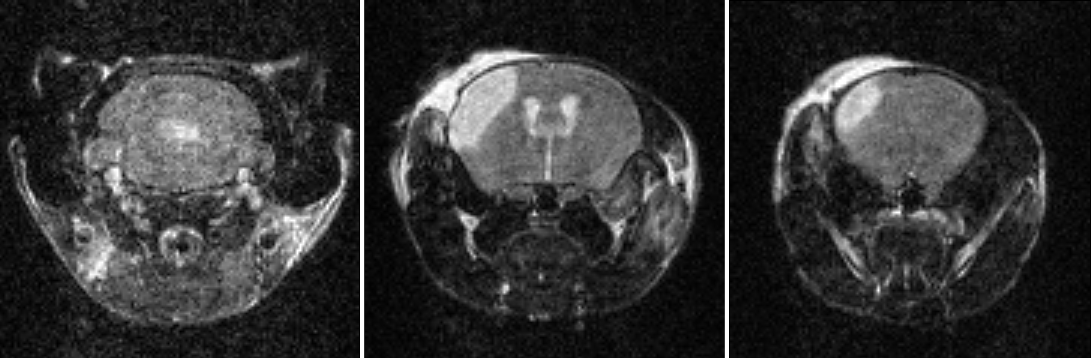
\includegraphics[width=0.8\textwidth]{Imagenes/Procesamiento/NiftyExample.png}
    \caption{Ejemplo de slices de IRM}
    \label{fig:img_slice}
\end{figure}

\subsection{Segmentación manual mediante ROI}

Una vez obtenidos los volúmenes en formato NIfTI, se procede a la segmentación manual de las estructuras de interés mediante la definición de regiones de interés (ROI). Este proceso ha sido realizado utilizando las herramientas \textit{MRIFIleManager} junto con la libreria \textit{ImageJ}, siguiendo el manual de uso y bajo la supervisión de expertos del centro ICTS BioImagen Complutense.

Las ROI se definen como contornos sobre cada \textit{slice}, delimitando tanto el cerebro completo como las regiones afectadas por isquemia. Este proceso requiere una interpretación visual experta, especialmente en el caso de las lesiones isquémicas, donde los bordes no están claramente definidos y existen gradientes de intensidad.
Como consecuencia, las anotaciones presentan un cierto grado de subjetividad, lo cual constituye una limitación inherente al problema abordado.
\begin{figure}[h]
    \centering
    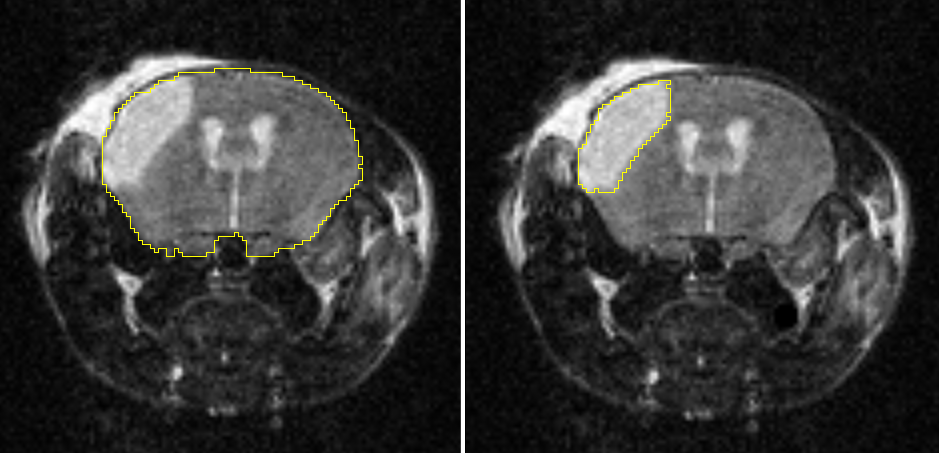
\includegraphics[width=0.8\textwidth]{Imagenes/Procesamiento/SegmentationExaple.png}
    \caption{Ejemplo de segmentación ROI}
    \label{fig:img_roi}
\end{figure}

\subsection{Generación de máscaras binarias}

A partir de las anotaciones ROI, se generan máscaras binarias que representan la información de segmentación en un formato adecuado para el entrenamiento supervisado.

Este proceso ha sido implementado mediante un script específico desarrollado en Python, que permite transformar las regiones definidas por contornos en imágenes discretas binarias alineadas con las slices originales. En estas máscaras, cada píxel se etiqueta como fondo (valor 0) o región de interés (valor 255), garantizando la correspondencia espacial con la imagen de entrada.

Adicionalmente, el script realiza las operaciones de adaptación necesarias para el entrenamiento del modelo, incluyendo el redimensionado de las imágenes y máscaras a una resolución uniforme(120px x 120px), así como la interpolación correspondiente. Este paso es crítico para asegurar la coherencia dimensional del dataset y su compatibilidad con la arquitectura de la red neuronal empleada.

El desarrollo de esta herramienta ha permitido automatizar el proceso de generación de \textit{ground truth}, asegurando la consistencia del dataset y reduciendo posibles errores derivados de la intervención manual. Asimismo, facilita la reutilización del pipeline por parte de usuarios con menor experiencia técnica, permitiendo la generación de nuevos conjuntos de entrenamiento y el reentrenamiento de los modelos de forma más accesible. \citep{repositorio_github}

\begin{figure}[h]
    \centering
    
\includegraphics[width=0.8\textwidth]{Imagenes/Procesamiento/BinaryExample.png}
    \caption{Ejemplo de máscara binaria}
    \label{fig:img_binary}
\end{figure}


\subsection{Normalización y adaptación de las imágenes}

Con el objetivo de garantizar la homogeneidad de los datos de entrada, las imágenes y sus máscaras son sometidas a un proceso de adaptación previo al entrenamiento.

En primer lugar, todas las imágenes son redimensionadas a una resolución de 120x120 píxeles. Esta decisión permite adaptar los datos a la arquitectura de la red neuronal empleada y reducir el coste computacional.

Durante este proceso se aplica interpolación, lo que puede introducir suavizado en los bordes y pérdida de detalle en estructuras pequeñas.

Asimismo, las intensidades de las imágenes, originalmente almacenadas en formato entero (\texttt{int16}), se convierten a formato de coma flotante (\texttt{float32}) y se normalizan para estabilizar el proceso de entrenamiento.

Por último, tanto las máscaras de entrenamiento como las slices de la IRM se orientan y se muestra una superposición para asegurar que el entrenamiento va a realizarse de manera correcta, alineando la máscara de entrenamiento con el órgano.

\begin{figure}[h]
    \centering
    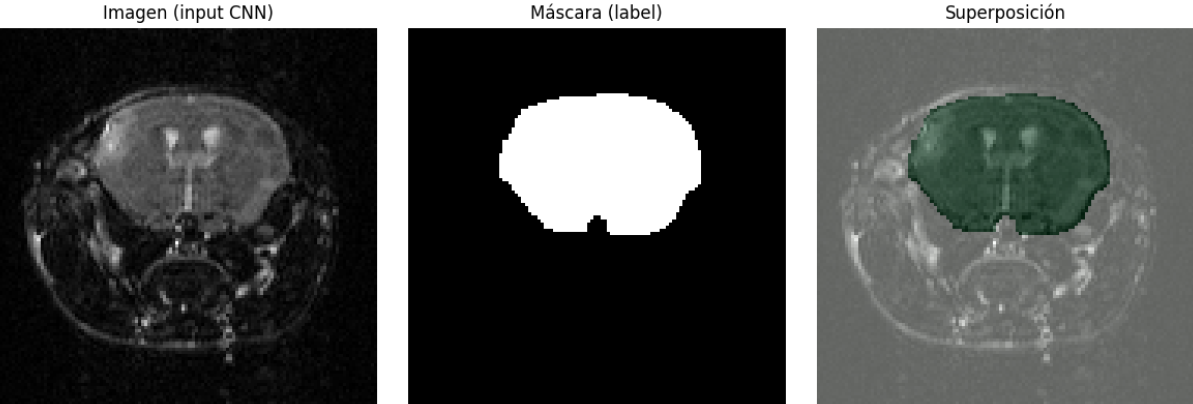
\includegraphics[width=0.8\textwidth]{Imagenes/Procesamiento/SuperpositionExample.png}
    \caption{Visualización de superposición de máscaras}
    \label{fig:img_mask}
\end{figure}
\section{Arquitectura de los modelos y \textit{Transfer Learning}}

Tras realizar un preprocesamiento de las imágenes para su uso en el entrenamiento, procedemos a definir la arquitectura a alto nivel de la aplicación de segmentación automática. En el caso de estudio que nos presenta ICTS BioImagen Complutense, se requiere la automatización de la medición de volúmenes de la lesión isquémica en el cerebro, además de la afectación en este órgano; por lo que es necesaria la segmentación automática por separado del órgano y de la lesión.

Para esta tarea, se utiliza la arquitectura U-Net para crear dos modelos, entrenados con las mismas imágenes pero con distintas máscaras binarias. Aunque existen múltiples variantes de U-Net, como U-Net++, Attention U-Net o ResUNet, se decide usar U-Net como estructura básica, teniendo en cuenta ventajas e inconvenientes relacionados con la complejidad técnica, la capacidad del modelo y el coste computacional, que se expondrán más adelante en esta sección.

Debido al bajo número de datos anotados, habitual en el ámbito biomédico, se aplica además \textit{Transfer Learning}, una técnica de \textit{Deep Learning} que permite reutilizar pesos previamente aprendidos por otros modelos para adaptarlos a una tarea más concreta. Para ello, se emplean pesos de \textit{RadImageNet}, un modelo preentrenado con IRM, TAC y ecografía.

Tras los primeros entrenamientos, se observó una tendencia a la sobresegmentación en el modelo de isquemia. Para mitigar este problema, se probaron varias estrategias, como el cambio de la función de pérdida para penalizar los falsos positivos. Finalmente, se optó por ajustar el umbral de binarización de la salida probabilística del modelo. La comparación cuantitativa de los distintos umbrales se presenta en el capítulo de resultados.

Además, se contempla la aplicación de técnicas de Inteligencia Artificial Explicable para proporcionar robustez al análisis, verificar que el modelo basa sus predicciones en regiones anatómica y patológicamente relevantes, y mejorar la confianza en los resultados obtenidos.

\subsection{Arquitectura U-Net y decisiones de implementación}

La arquitectura principal empleada en este trabajo para la segmentación automática se basa en una U-Net 2D, la cual se repite en los dos modelos desarrollados (cerebro e isquemia). En nuestro caso, esta arquitectura se adaptó para trabajar con cortes bidimensionales de resonancia magnética preclínica, de manera que cada muestra de entrada se representa como una imagen en escala de grises redimensionada a \(120 \times 120\) píxeles. Además, dado que el encoder seleccionado requiere tres canales de entrada, cada imagen monocanal se replicó tres veces antes de ser introducida en la red.

A nivel estructural, la red mantiene el esquema clásico encoder--decoder característico de U-Net. En la rama contractiva, el encoder \texttt{ResNet50} actúa como extractor jerárquico de características, generando representaciones cada vez más abstractas de la imagen de entrada conforme aumenta la profundidad de la red. A su vez, a partir del encoder se obtienen varios mapas de características intermedios que posteriormente se reutilizan en el decoder a través de conexiones de salto, preservando así información espacial de alta resolución, necesaria para obtener una segmentación precisa \citep{ronneberger2015unet}. En la rama expansiva, la máscara de salida se reconstruye mediante varias etapas sucesivas de sobremuestreo y concatenación con estos mapas intermedios.

En la implementación del decoder se optó por una estrategia de sobremuestreo mediante \texttt{UpSampling2D} seguida de convoluciones convencionales, en lugar de utilizar convoluciones transpuestas. Esta decisión permite separar el aumento de resolución del refinamiento de características y ayuda a reducir la aparición de artefactos tipo \textit{checkerboard}\footnote{
Los artefactos \textit{checkerboard} son patrones visuales no deseados con apariencia de cuadrícula o tablero de ajedrez, que pueden aparecer en imágenes generadas o reconstruidas mediante ciertas operaciones de convolución transpuesta.
}, asociados a ciertas configuraciones de deconvolución \citep{odena2016deconvolution}.

En cuanto a la salida del modelo, esta se obtiene mediante una convolución \(1 \times 1\) con activación sigmoidal, lo que permite generar una máscara binaria de probabilidad por píxel para la clase objetivo. Esta formulación es coherente con el problema planteado, ya que tanto la segmentación del cerebro como la de la lesión se modelan como tareas de segmentación binaria, donde cada píxel debe clasificarse como perteneciente o no a la región de interés.

Como se muestra en la Figura \ref{fig:arquitectura_unet}, ambos modelos comparten la misma arquitectura base, diferenciándose únicamente en la máscara objetivo empleada durante el entrenamiento: uno orientado a la segmentación del cerebro y el otro hacia la segmentación de la lesión isquémica. La figura muestra la entrada de tamaño \(120 \times 120 \times 3\), el encoder \texttt{ResNet50} preentrenado sobre \textit{RadImageNet}, las conexiones de salto, el decoder basado en \texttt{UpSampling2D} y convoluciones, y la generación de la máscara binaria de salida. Esta misma arquitectura base se utiliza tanto para el modelo de segmentación de cerebro como para el de segmentación de isquemia, diferenciándose únicamente en la máscara objetivo empleada durante el entrenamiento.

\begin{figure}[htbp]
    \centering
    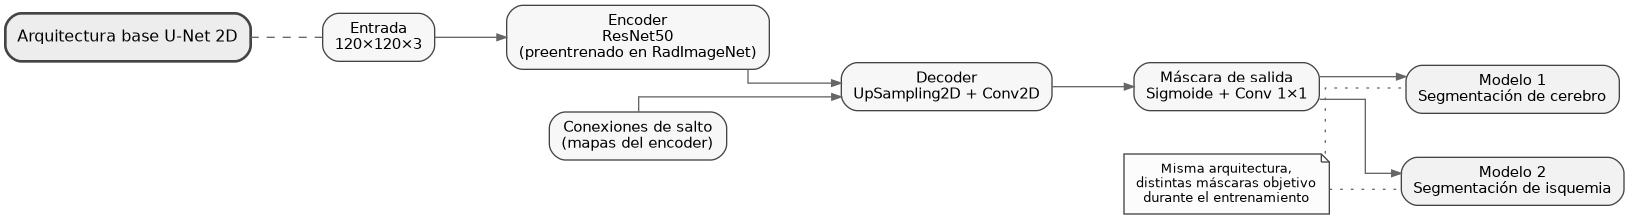
\includegraphics[width=0.95\textwidth]{Imagenes/Bitmap/arquitectura_unet_es.gv.png}
    \caption{Esquema de la arquitectura U-Net 2D empleada en este trabajo.}
    \label{fig:arquitectura_unet}
\end{figure}
\subsection{Justificación de la arquitectura y uso de \textit{Transfer Learning}}

Aunque existen variantes más complejas de esta arquitectura, como U-Net++ \citep{zhou2018unetplusplus} o Attention U-Net \citep{oktay2018attentionunet}, se decide utilizar U-Net como estructura base del sistema. Esta elección se toma teniendo en cuenta que, aunque estas variantes introducen mejoras interesantes a nivel arquitectónico, también aumentan la complejidad del modelo y el número de elementos a ajustar durante el entrenamiento. En este caso, al trabajar con un conjunto de datos reducido y dentro del alcance de un TFG, resulta más razonable partir de una arquitectura ya consolidada en segmentación biomédica, suficientemente robusta y más sencilla de controlar experimentalmente \citep{ronneberger2015unet}. De este modo, en lugar de añadir complejidad desde la propia arquitectura, se opta por mantener una U-Net base y reforzarla mediante \textit{Transfer Learning}, buscando así un equilibrio entre capacidad de segmentación, coste computacional y facilidad de implementación.

De esta manera se opta por aplicar \textit{Transfer Learning}: una técnica de \textit{Deep Learning} especialmente útil cuando no se dispone de un conjunto de entrenamiento lo suficientemente grande como para entrenar un modelo profundo desde cero. Para ello, se incorporó un encoder \texttt{ResNet50} preentrenado con pesos de \textit{RadImageNet}, con el objetivo de partir de una base de conocimiento visual ya aprendida en imagen médica, en lugar de comenzar con una inicialización aleatoria de los pesos. Esta decisión está respaldada por el trabajo de \citep{mei2022radimagenet}, donde se muestra que los modelos preentrenados en \textit{RadImageNet} pueden servir como un punto de partida eficaz para tareas posteriores de imagen biomédica. De este modo, la U-Net implementada en este trabajo no parte de un encoder entrenado desde cero, sino de un backbone previamente adaptado al dominio radiológico, lo que refuerza la justificación de esta elección.

En conjunto, ambas decisiones responden a una misma necesidad: disponer de un modelo con suficiente capacidad de representación para segmentar estructuras biomédicas complejas, pero que al mismo tiempo pueda entrenarse de forma estable en un contexto de datos limitados, por lo que el uso de \textit{Transfer Learning} resulta una estrategia adecuada para alcanzar este objetivo.

\subsection{Estrategia de entrenamiento y ajuste de la salida}

Para el proceso de entrenamiento, se siguió una estrategia en dos fases: en una primera etapa, el encoder preentrenado permaneció congelado y únicamente se entrenó la parte decodificadora de la red, de forma que el modelo pudiera adaptarse a la tarea concreta sin modificar las representaciones aprendidas previamente. En una segunda etapa, se descongelaron las últimas capas del encoder para realizar un ajuste fino controlado del modelo completo. Con ello se buscó mantener el conocimiento transferido desde el preentrenamiento, permitiendo al mismo tiempo cierta especialización del extractor de características al dominio concreto de la imagen de IRM.

La función de pérdida seleccionada fue una combinación de entropía cruzada binaria y pérdida Dice (\texttt{BCE + Dice loss}). Esta elección se tomó debido a que permite optimizar simultáneamente dos aspectos importantes de la segmentación: por un lado, la clasificación correcta de cada píxel de forma individual y, por otro lado, el grado de solapamiento global entre la máscara predicha y la máscara de referencia.

Mientras que la componente BCE penaliza errores locales de clasificación, la componente Dice resulta especialmente útil en segmentación médica cuando existe un claro desbalance entre fondo y región objetivo, como ocurre con frecuencia en la delimitación de lesiones pequeñas \citep{milletari2016vnet}. Como métrica principal de seguimiento durante el entrenamiento se utilizó el coeficiente Dice, por ofrecer una medida directa del grado de coincidencia entre la segmentación automática y la segmentación manual.

A nivel de configuración, el entrenamiento se realizó con el optimizador Adam y un tamaño de lote de 4. En la primera fase se utilizó una tasa de aprendizaje de \(10^{-4}\), que posteriormente se redujo a \(10^{-5}\) durante la fase de ajuste fino del encoder. En total, el entrenamiento quedó estructurado en 25 épocas con el encoder congelado y 10 épocas adicionales de \textit{fine-tuning}, incorporando además una partición de validación para monitorizar la evolución del modelo y seleccionar configuraciones estables.

\begin{table}[h]
\centering
\caption{Configuración general del entrenamiento de los modelos de segmentación.}
\label{tab:config_entrenamiento}
\begin{tabular}{ll}
\hline
Parámetro & Valor \\
\hline
Arquitectura base & U-Net 2D con encoder \texttt{ResNet50} \\
Tamaño de entrada & \(120 \times 120 \times 3\) \\
Optimizador & Adam \\
Tamaño de lote & 4 \\
Función de pérdida & BCE + Dice Loss \\
Métrica principal & Coeficiente Dice \\
Tasa de aprendizaje (fase 1) & \(10^{-4}\) \\
Tasa de aprendizaje (fase 2) & \(10^{-5}\) \\
Épocas con encoder congelado & 25 \\
Épocas de \textit{fine-tuning} & 10 \\
Salida del modelo & Máscara probabilística con activación sigmoidal \\
\hline
\end{tabular}
\end{table}

Tras los primeros experimentos con el modelo de isquemia, se observó que el umbral de binarización influía de forma directa tanto en la calidad espacial de la segmentación como en la precisión de la cuantificación volumétrica. Por ello, durante la fase de validación se evaluaron distintos valores de umbral, con el objetivo de seleccionar una configuración adecuada para la inferencia final.

Este ajuste se consideró especialmente relevante en el modelo de isquemia, ya que la lesión ocupa una región reducida respecto al fondo y el modelo puede generar falsos positivos en zonas de baja probabilidad. En cambio, en el modelo de segmentación cerebral no se introdujo un ajuste específico del umbral, al tratarse de una estructura anatómica de mayor tamaño y con una segmentación más estable.

Finalmente, para el modelo de isquemia se adoptó un umbral de binarización de \(0.80\) en la fase de inferencia. La comparación cuantitativa de los umbrales evaluados, así como la justificación experimental del valor finalmente seleccionado, se presentan en el capítulo de resultados.

\section{Cuantificación y métricas biomédicas (volumen)}

La segmentación automática proporciona una delimitación espacial del cerebro y de la lesión isquémica. Sin embargo, para que esta salida sea útil en un contexto de investigación biomédica, es necesario transformarla en magnitudes cuantitativas que permitan comparar casos y evaluar diferencias entre segmentaciones manuales y automáticas.

En este trabajo, la métrica cuantitativa principal es el volumen de las regiones segmentadas. Esta magnitud permite estimar la extensión del órgano y de la lesión, facilitando el análisis posterior de los casos estudiados. En el ámbito de la imagen cerebral, y en particular en estudios de ictus, el volumen lesional se utiliza habitualmente como una medida relevante para caracterizar la afectación observada en resonancia magnética \citep{Harston2015,Ospel2024}.

Para realizar esta cuantificación, se toma como entrada la salida del \textit{pipeline} de segmentación. Dicha salida consiste en una máscara binaria asociada a cada corte de la resonancia magnética, donde los píxeles con valor positivo representan la región segmentada y el resto corresponde al fondo o a zonas no incluidas en la segmentación.

Dado que las imágenes médicas se almacenan en formato NIfTI, el volumen no se calcula únicamente a partir del número de píxeles segmentados, sino teniendo en cuenta la información espacial de la imagen. En este formato, el campo \texttt{pixdim} codifica el espaciado físico de la rejilla en cada dimensión, mientras que la información \textit{affine} (\texttt{sform}/\texttt{qform}) permite representar la geometría espacial asociada a la imagen \citep{NIfTI1Fields,NiBabelNifti}. De este modo, si \(N\) representa el número total de vóxeles segmentados, y \(s_x\), \(s_y\) y \(s_z\) representan el tamaño físico del vóxel en cada una de las tres dimensiones espaciales, el volumen total puede expresarse como:

\begin{equation}
V = N \cdot s_x \cdot s_y \cdot s_z
\end{equation}

donde:

\begin{itemize}
    \item \(V\) es el volumen total de la región segmentada,
    \item \(N\) es el número total de vóxeles clasificados como pertenecientes al órgano o a la lesión,
    \item \(s_x\) y \(s_y\) corresponden a la resolución espacial en el plano de la imagen,
    \item \(s_z\) corresponde al espesor del corte, expresado en unidades físicas.
\end{itemize}

En la práctica, como la segmentación se obtiene corte a corte, el cálculo también puede formularse como la suma del volumen parcial aportado por cada corte. Si \(A_i\) representa el área segmentada en el corte \(i\), el volumen total se obtiene como:

\begin{equation}
V = \sum_{i=1}^{n} A_i \cdot s_z
\end{equation}

siendo \(n\) el número total de cortes segmentados. A su vez, el área segmentada en cada corte puede calcularse como:

\begin{equation}
A_i = N_i \cdot s_x \cdot s_y
\end{equation}

donde \(N_i\) es el número de píxeles segmentados en el corte \(i\).

La Figura~\ref{fig:calculo_volumen_lesion} resume este procedimiento. Para cada corte, se contabilizan los píxeles pertenecientes a la región de interés y se transforman en un área física utilizando la resolución espacial de la imagen en el plano \((s_x, s_y)\). Posteriormente, la suma de las áreas segmentadas se combina con el espaciado entre cortes \((s_z)\) para estimar el volumen total.

\begin{figure}[htbp]
    \centering
    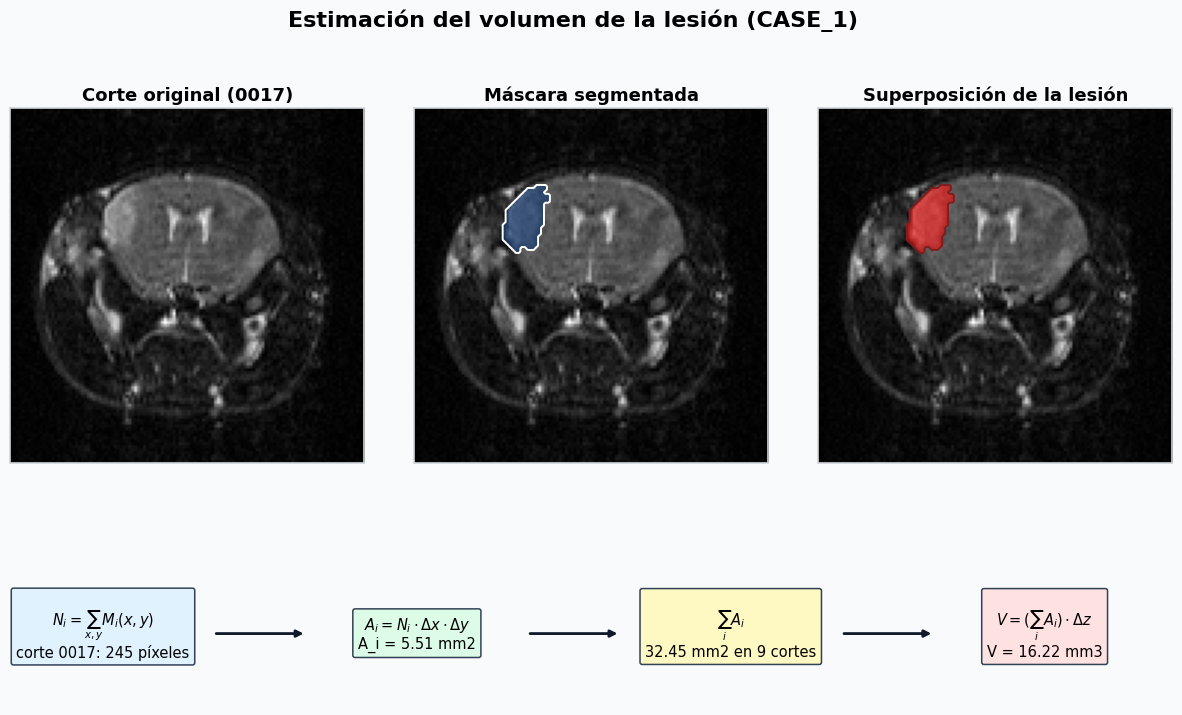
\includegraphics[width=\textwidth]{Imagenes/Bitmap/calculo_volumen.png}
    \caption{Proceso de cálculo del volumen de la lesión a partir de la máscara segmentada.}
    \label{fig:calculo_volumen_lesion}
\end{figure}

Este procedimiento permite transformar la salida binaria del modelo en una medida físicamente interpretable, expresada en milímetros cúbicos (\(\text{mm}^3\)). El uso de unidades físicas, en lugar de recuentos de píxeles sin escala, resulta esencial para que las medidas obtenidas sean comparables entre diferentes resonancias, sujetos y estudios experimentales.

Desde el punto de vista metodológico, la cuantificación volumétrica amplía la utilidad del sistema desarrollado, ya que la herramienta no solo proporciona una segmentación visual de la región de interés, sino también una medida numérica objetiva. Esta salida resulta coherente con el flujo de trabajo que se busca automatizar en ICTS BioImagen Complutense, donde la segmentación manual de las regiones de interés se utiliza posteriormente para estimar volúmenes y analizar la afectación observada. Además, este enfoque coincide con otros trabajos de segmentación biomédica orientados a la medición automática de carga lesional en resonancia magnética \citep{Oliveira2022,Akkus2017}.

\section{Integración de explicabilidad}

Desde el inicio de este Trabajo de Fin de Grado, uno de los objetivos del proyecto no solo implicaba el desarrollo del \textit{pipeline} de segmentación y cálculo de volúmenes, sino también el análisis de la robustez y la interpretabilidad de los modelos. La aplicación de modelos de \textit{deep learning} a una tarea realizada habitualmente por expertos introduce el riesgo de incorporar un proceso de caja negra en un contexto, como el biomédico, donde la transparencia resulta especialmente relevante para generar confianza en los resultados y facilitar su análisis crítico \citep{samek2017explainableartificialintelligenceunderstanding,doshivelez2017rigorousscienceinterpretablemachine}.

En este apartado se expone la metodología seguida para integrar técnicas de Inteligencia Artificial Explicable (XAI) en los dos modelos que forman parte del \textit{pipeline} de segmentación automática. Dado que los fundamentos de los métodos empleados ya se han descrito en el estado de la cuestión, esta sección se centra en su adaptación práctica al problema de segmentación y en cómo se incorporan al flujo de análisis desarrollado.

\subsection{Motivación de la explicabilidad en el sistema}

Aunque los resultados de segmentación pueden evaluarse mediante métricas cuantitativas, estas no son suficientes para comprender cómo se generan las predicciones del modelo. Una segmentación puede obtener buenos valores de solapamiento y, aun así, apoyarse en patrones no deseados, artefactos de adquisición o regiones anatómicas no relacionadas con la estructura de interés.

Este aspecto resulta especialmente relevante en imagen biomédica, donde el objetivo no es únicamente obtener una máscara precisa, sino también comprobar que el comportamiento del modelo sea coherente con el dominio de aplicación. Además, el uso de un conjunto de datos reducido incrementa la probabilidad de que la red aprenda relaciones poco generalizables, por lo que la explicabilidad se incorpora como una herramienta complementaria para analizar el comportamiento interno del sistema.

En este trabajo, la explicabilidad se utiliza con dos objetivos principales. En primer lugar, permite generar mapas de relevancia que indican qué zonas de la imagen contribuyen en mayor medida a la salida del modelo. En segundo lugar, facilita el análisis crítico de las segmentaciones obtenidas, al permitir estudiar si la red se apoya en regiones anatómicamente coherentes o si aparecen dependencias no deseadas en zonas externas a la región de interés.

\subsection{Adaptación de XAI a modelos de segmentación}

Una de las principales dificultades al aplicar técnicas de explicabilidad en este trabajo es que muchos métodos de XAI fueron diseñados originalmente para tareas de clasificación. En estos problemas, la salida del modelo suele ser un valor escalar asociado a una clase concreta. Sin embargo, en segmentación, la salida del modelo es una máscara densa, donde cada píxel tiene asociada una probabilidad de pertenencia a la clase objetivo.

Por este motivo, no es posible aplicar directamente estos métodos sin realizar una adaptación previa. Para ello, se define una función de \textit{score} escalar a partir de la salida del modelo. Esta función resume la predicción densa en un único valor, sobre el que pueden calcularse gradientes o perturbaciones de forma compatible con las técnicas de explicabilidad utilizadas.

En este trabajo, el \textit{score} se define a partir de la activación del modelo en la región segmentada por la propia red. De este modo, la explicación no se calcula sobre una clase global de imagen, sino sobre la región que el modelo ha identificado como perteneciente a la estructura objetivo. Esta decisión permite adaptar métodos originalmente propuestos para clasificación al contexto de segmentación biomédica.

El cálculo se realiza sobre la predicción del modelo y no sobre la máscara de referencia. Esta decisión es importante, ya que el objetivo de la explicabilidad no es medir directamente la coincidencia con la anotación manual, sino analizar qué información utiliza la red para generar su propia salida.

\subsection{Procedimiento de integración en el \textit{pipeline}}

La explicabilidad se integra como una fase posterior a la inferencia de los modelos de segmentación. Una vez obtenidas las máscaras predichas, se generan mapas de relevancia asociados a la salida de cada modelo. Para ello, se han implementado notebooks específicos que cargan los modelos entrenados, procesan los volúmenes de resonancia magnética corte a corte y reproducen el mismo flujo seguido durante la inferencia.

En el caso del modelo de isquemia, el procedimiento mantiene la estructura secuencial del \textit{pipeline}: primero se obtiene la máscara cerebral, después se utiliza dicha máscara para restringir la entrada al tejido cerebral y, finalmente, se genera la predicción de lesión. A partir de esta salida se calculan los mapas de relevancia asociados a la región segmentada como isquemia.

En el caso del modelo de segmentación cerebral, el procedimiento se aplica directamente sobre la predicción de cerebro generada por el modelo. La explicación se calcula sobre la región que la red identifica como tejido cerebral, con el objetivo de estudiar si la predicción depende de zonas coherentes con la estructura anatómica segmentada.

Aunque cada modelo tiene una región objetivo distinta, el marco de explicabilidad empleado es común. En ambos casos se parte de la salida probabilística del modelo, se define un \textit{score} escalar sobre la región predicha y se calculan los mapas de relevancia correspondientes. Posteriormente, estos mapas se normalizan y se redimensionan al tamaño de la imagen de entrada para facilitar su visualización junto con el corte original, la máscara de referencia y la máscara predicha.

Para los métodos basados en Grad-CAM, se selecciona la última capa convolucional del decoder, previa a la convolución final \(1 \times 1\), al tratarse de una capa cercana a la generación de la máscara de salida y que todavía conserva información espacial relevante. Esta elección permite obtener mapas de activación relacionados con la decisión final del modelo sin perder completamente la estructura espacial de la imagen.

Además de los mapas visuales, se incorporan métricas basadas en perturbación de la entrada, como \textit{Deletion}, \textit{Insertion} y AOPC. Estas métricas se emplean para estudiar si las regiones identificadas como relevantes tienen influencia real sobre la salida del modelo, complementando así la interpretación visual de los mapas de relevancia \citep{samek2017evaluating,petsiuk2018rise}.

Cabe destacar que los mapas de relevancia no deben interpretarse como segmentaciones adicionales ni como una validación clínica directa. Su función es proporcionar una aproximación al comportamiento interno del modelo, permitiendo analizar qué regiones de la imagen influyen en la predicción. Por tanto, la explicabilidad se plantea como una herramienta complementaria a las métricas de segmentación y a la evaluación volumétrica.

Los resultados visuales y cuantitativos derivados de esta integración se presentan posteriormente en el capítulo de resultados, donde se analizan ejemplos representativos para ambos modelos y se discute la coherencia de las explicaciones obtenidas.

\section[Implementación y reproducibilidad]{Implementación, reproducibilidad y código entregado}

El desarrollo práctico del programa se ha organizado en una serie de notebooks de \textit{Python}, que constituyen el código entregado junto con esta memoria. Esta decisión se corresponde con el carácter experimental del proyecto y con la necesidad de documentar de forma clara cada fase del flujo de trabajo: entrenamiento, inferencia, cálculo de métricas y explicabilidad.

El uso de notebooks resulta adecuado en este contexto por varios motivos. En primer lugar, permite combinar código, explicaciones intermedias, visualizaciones y resultados en un mismo entorno, facilitando la revisión del proceso seguido. En segundo lugar, favorece la reproducibilidad, ya que cada notebook puede ejecutarse de forma secuencial y permite comprobar de manera directa las entradas, salidas y transformaciones aplicadas en cada etapa. Además, durante el desarrollo del TFG se acordó mantener el sistema en formato notebook, sin interfaz gráfica independiente, siempre que estos incluyeran de forma clara el procedimiento de entrenamiento, uso y evaluación de los modelos.

Esta organización también facilita el uso del sistema por parte de usuarios no especializados en desarrollo software, especialmente en entornos como Google Colab o Jupyter Notebook. De este modo, el usuario puede ejecutar el flujo de trabajo por bloques, modificar parámetros concretos y visualizar los resultados sin necesidad de desplegar una aplicación completa. Por tanto, los notebooks no se plantean únicamente como scripts de desarrollo, sino como una forma documentada y ejecutable de entregar el prototipo.

Por lo tanto, se entregan cinco notebooks principales, cada uno de ellos con responsabilidades diferenciadas. En primer lugar, el notebook de entrenamiento, \path{UNET_RadImageNet_unificado.ipynb}, contiene la definición de la arquitectura U-Net empleada, la carga del conjunto de datos, el preprocesamiento de las imágenes y máscaras, la configuración de entrenamiento y el guardado final de los modelos. Este notebook permite reproducir el proceso de entrenamiento, pudiéndose entrenar un único modelo para una tarea concreta o dos modelos, uno de órgano y otro de lesión. En este último caso, se aplica la máscara de \textit{Ground Truth} del órgano sobre la imagen original, de forma que el modelo de lesión se entrena únicamente sobre la región anatómica correspondiente.

Se adjunta además un notebook de testeo, \path{Tester_Pipeline.ipynb}, que permite cargar los modelos entrenados y ejecutar el \textit{pipeline} completo. En primer lugar, se cargan los modelos y el caso de estudio a analizar. A continuación, se obtiene la máscara del órgano, se restringe la imagen original a dicha región y se aplica el modelo de lesión. Finalmente, las máscaras resultantes se utilizan para calcular los volúmenes de órgano y lesión. Este notebook permite reproducir el proceso de inferencia, obteniendo tanto las máscaras segmentadas como los volúmenes cuantificados a partir de la imagen de entrada.

El notebook \path{GraphTester.ipynb} contiene el código utilizado para generar las métricas de los modelos, expuestas posteriormente en el capítulo de resultados. En este notebook se implementan las funciones necesarias para calcular el coeficiente Dice, el error absoluto de volumen y el error relativo porcentual, tanto a nivel de corte como a nivel volumétrico. Además, se incluyen funciones para generar gráficos comparativos entre la segmentación automática y la manual, facilitando la visualización de los resultados obtenidos.

Los notebooks de XAI para el cerebro y la lesión isquémica implementan el análisis de explicabilidad de los modelos entrenados. Ambos siguen una estructura común: carga del modelo, selección de la capa objetivo, generación de mapas de relevancia, cálculo de métricas de fidelidad y exportación de resultados. En ellos se aplican técnicas como Grad-CAM, Grad-CAM++, \textit{Integrated Gradients} y oclusión. Además, se generan curvas de perturbación como \textit{Deletion}, \textit{Insertion}, MoRF y LeRF, junto con métricas derivadas como AOPC. Estos resultados se exportan en formato CSV y como figuras, facilitando su incorporación al análisis cualitativo y cuantitativo de la memoria.

Además, se incluyen los dos modelos desarrollados, guardados en formato \texttt{.h5}, que pueden ser cargados directamente para realizar el proceso de inferencia sobre nuevos casos de estudio. Estos modelos corresponden a la arquitectura U-Net entrenada para segmentar el cerebro y la lesión isquémica, respectivamente.

Por último, también se adjuntan, como parte de la reproducibilidad del proyecto, los archivos resultantes de la ejecución de los notebooks de cálculo de métricas y explicabilidad, con los datos resultantes en formato CSV y las imágenes generadas en formato PNG.

\subsection{Requisitos de ejecución}

Para facilitar la reproducción del trabajo, el código se ha organizado de forma que pueda ejecutarse en un entorno estándar de \textit{Python}, preferiblemente mediante Jupyter Notebook o Google Colab. No se requiere una infraestructura específica ni software propietario para ejecutar la inferencia o el cálculo de métricas, aunque el entrenamiento de los modelos puede beneficiarse del uso de GPU para reducir el tiempo de ejecución.

Los requisitos principales del entorno son los siguientes:

\begin{itemize}
    \item Un entorno de ejecución compatible con notebooks, como Jupyter Notebook, JupyterLab o Google Colab.
    \item Python 3.x, junto con las librerías necesarias para procesamiento de imagen, aprendizaje profundo, lectura de volúmenes médicos y visualización de resultados.
    \item Acceso a los modelos entrenados en formato \texttt{.h5}, en caso de ejecutar únicamente la inferencia.
    \item Imágenes de entrada en formato NIfTI, organizadas según la estructura de carpetas descrita en la sección del conjunto de datos.
    \item Máscaras de referencia, en caso de reproducir el entrenamiento o calcular métricas comparativas frente a segmentaciones manuales.
\end{itemize}

Entre las librerías utilizadas se incluyen TensorFlow/Keras para la definición, entrenamiento y carga de los modelos; NumPy y Pandas para el tratamiento de datos; NiBabel para la lectura de imágenes médicas en formato NIfTI; Pillow y OpenCV para operaciones de preprocesamiento de imagen; Matplotlib y Plotly para la generación de figuras y visualizaciones; y Scikit-learn para funciones auxiliares de evaluación. Las dependencias concretas del proyecto deben recogerse en un fichero \texttt{requirements.txt} dentro del repositorio, de forma que el entorno pueda reconstruirse mediante instalación automática.

\begin{table}[H]
\centering
\small
\renewcommand{\arraystretch}{1.2}
\begin{tabularx}{\textwidth}{p{0.28\textwidth} X}
\hline
\textbf{Requisito} & \textbf{Descripción} \\
\hline

Entorno de ejecución &
Jupyter Notebook, JupyterLab o Google Colab. \\

Lenguaje &
Python 3.x. \\

Aprendizaje profundo &
TensorFlow/Keras para entrenamiento, carga e inferencia de los modelos. \\

Procesamiento de datos &
NumPy y Pandas para manipulación de matrices, métricas y exportación de resultados. \\

Imagen médica &
NiBabel para lectura de volúmenes NIfTI y acceso a la información espacial de la imagen. \\

Procesamiento de imagen &
Pillow y OpenCV para redimensionado, normalización y manipulación de máscaras. \\

Visualización &
Matplotlib y Plotly para generación de gráficas, máscaras, mapas de calor y figuras exportables. \\

Archivos necesarios &
Modelos \texttt{.h5}, imágenes NIfTI de entrada y, cuando proceda, máscaras manuales de referencia. \\

\hline
\end{tabularx}
\caption{Requisitos principales para la ejecución y reproducción del código entregado.}
\label{tab:requisitos_codigo}
\end{table}

\subsection{Repositorio y estructura del código entregado}

Todo el código desarrollado se encuentra disponible en el repositorio de GitHub del proyecto:

\begin{center}
\url{https://github.com/beabuenodev/Herramienta-de-Analisis-de-Imagenes-Biomedicas}
\end{center}